\section{Results}\label{sec:results}

\subsection{Measurement protocol}\label{sec:measure}

Each system--strategy pair was run $R$ times with fixed random seeds: $R=100$ for levels A and B, the synthetic families, and the ablation; $R=50$ for the stagger-and-step, hyperparameter, horizon, bisection, and enlarged-region tests; and $R=10$--$100$ for the coupled systems. A run stops at the first hit or when the budget is exhausted. The first 50 points of all strategies coincide with the first 50 points of uniform sampling (common random numbers). The cost $N_{0.9}$ is the linearly interpolated 0.9 quantile of the first-hit index over the runs (infinite if fewer than 90\% of the runs find the target), with 95\% bootstrap percentile intervals~\cite{EfronTibshirani1994} over 2000 resamples of the runs of the strategy and of the uniform reference. The exponent $s$ is the slope of the regression of $\ln N_{0.9}$ on $\ln(1/p)$. Within each experiment, $N^0_{0.9}$ is remeasured by uniform sampling with the same $R$ and seeds, so the uniform costs in different tables differ by sampling error. So do the basin measures: the table of \cref{sec:rare_ab} takes them from the census of \cref{tab:benchmark}, whereas the other tables estimate them from their own uniform runs (for four uncoupled copies, $p=p_1^4$). The cost tables of \cref{sec:cost}, whose runs are few, and the stagger-and-step tests use a fixed reference per system. Uniform sampling for the coupled systems and the enlarged regions was run on a GPU with a kernel that reproduces the CPU trajectories and fingerprints bit for bit. Unless stated otherwise, a gain is a ratio of integration counts.

\subsection{Coupled copies: the gain is geometric in the number of units}\label{sec:coupled}

Coupling copies of a system with a hidden attractor yields a rare hidden target that is not constructed by hand: the regime in which every copy sits on its hidden attractor. We take $k$ copies of SE11 with mean-field coupling along $y$,
\begin{equation}
\dot{\bm x}_u=\bm F(\bm x_u)+\epsilon\,\bigl(\bar y-y_u\bigr)\,\bm e_y,\qquad u=1,\dots,k,\qquad \bar y=\frac1k\sum_{v}y_v,
\label{eq:coupled}
\end{equation}
in the region $B^k$, with $\epsilon=0.01$ or $\epsilon=0$. The only equilibrium is the synchronous equilibrium of SE11, which is stable, so the target regime is hidden. Its basin measure is $5.5\times10^{-5}$ for $k=2$ ($n=6$) and $3.5\times10^{-7}$ for $k=3$ ($n=9$), close to $p_1^k$ with $p_1=0.0079$, and it equals $p_1^4=3.9\times10^{-9}$ for four uncoupled copies ($n=12$).

\Cref{prop:product} predicts the gain from a single number characterizing one copy: the measure of its nonescaping set, $q=0.0472\pm0.0009$ from the census of $5\times10^4$ uniform points (the stable equilibrium takes 0.039 and the hidden attractor 0.0079; the rest escapes). The base of the geometric growth is $1/q=21.2$, the information bound for escape times is $2.56\,q^{-k}$, and the exponent of ideal splitting along $p=p_1^k$ is $s=1-\ln(1/q)/\ln(1/p_1)=0.37$. \Cref{tab:coupled} and \cref{fig:product} compare these predictions with the measured gains. The portfolio gains 65 at $n=6$, 1400--1600 at $n=9$, and $1.3\times10^4$ at $n=12$, where it needs $N_{0.9}=4.7\times10^4$ integrations instead of $5.9\times10^8$; all runs found the target. Over $k=2$--4, the gain grows geometrically with base 14.0 [10.7, 20.8] for the portfolio and 10.5 [7.7, 15.3] for splitting, against $1/q=21.2$; the cost exponent along the family is $s=0.42$ for the portfolio and $0.48$ for splitting, against the ideal $0.37$ and $1$ for uniform sampling. Every measured gain lies below the bound. The portfolio also observes regime labels and the settling part $D$, so the bound does not constrain it a priori; the fact that its gains stay below the bound and grow geometrically with a base of the predicted order shows that escape times are the dominant source of information on these systems. The gap to ideal splitting grows from a factor of 2 at $k=2$ to 14 at $k=4$, a loss of 1.5--2 per unit relative to exact sampling; part of it is structural, because ideal splitting needs $K_4=8$ levels at $k=4$, close to the cap of ten levels after which the implementation restarts. Coupling does not change the picture: with and without coupling at $n=9$, the gains agree within their intervals. Bisection toward basin boundaries does not scale on these systems: within budgets of $1.3\times10^5$ (about $7/p$) at $n=6$ and $2\times10^5$ at $n=9$, it finds the target in 66\% and 32\% of runs, respectively.

\begin{table}[tbhp]
\caption{Coupled copies of SE11, \eqref{eq:coupled}: basin measure of the regime ``all copies on the hidden attractor,'' cost of uniform sampling, measured gains $G_{0.9}$ with 95\% bootstrap intervals ($R=100$ for $n=3$ and for $n=9$ with coupling, $R=50$ otherwise), the gain of ideal splitting (Ideal) from \eqref{eq:Nk} with $n_0=50$, $p_0=0.2$, and the measured $q=0.0472$, and the information bound $2.56\,q^{-k}$ of \cref{prop:product}(i). For $n=12$, $N^0_{0.9}=\ln10/p_1^4$ is exact.}
\label{tab:coupled}
\centering\scriptsize
\setlength{\tabcolsep}{3pt}
\begin{tabular}{rrrrrr@{\hspace{12pt}}rr}
\toprule
$k$ ($n$) & $\epsilon$ & $p$ & $N^0_{0.9}$ & Splitting & Portfolio & Ideal & Bound \\
\midrule
1 (3) & --- & 0.0079 & 317 & 2.53 \ci{1.95}{2.86} & 3.10 \ci{2.46}{3.70} & 2.2 & 54 \\
2 (6) & 0.01 & $5.5\times10^{-5}$ & $3.8\times10^{4}$ & 44.0 \ci{27.0}{65.6} & 64.9 \ci{41.7}{86.6} & 129 & 1150 \\
3 (9) & 0.01 & $3.5\times10^{-7}$ & $7.6\times10^{6}$ & 682 \ci{448}{989} & 1435 \ci{896}{2372} & 9700 & $2.4\times10^{4}$ \\
3 (9) & 0 & $4.9\times10^{-7}$ & $5.3\times10^{6}$ & 598 \ci{325}{1000} & 1574 \ci{771}{2299} & 6800 & $2.4\times10^{4}$ \\
4 (12) & 0 & $3.9\times10^{-9}$ & $5.9\times10^{8}$ & 4881 \ci{3860}{6354} & 12\,681 \ci{9827}{18\,098} & $1.8\times10^{5}$ & $5.2\times10^{5}$ \\
\bottomrule
\end{tabular}
\end{table}

\begin{figure}[tbhp]
\centering
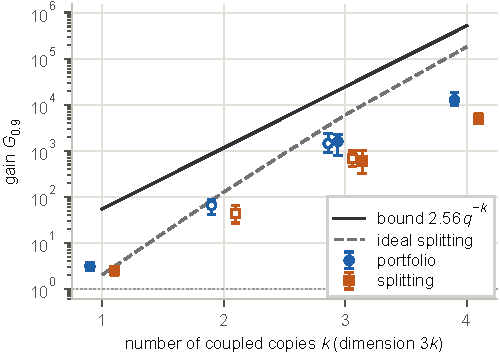
\includegraphics[width=0.62\textwidth]{fig_product_gain.pdf}
\caption{Gain on $k$ coupled copies of SE11 (\cref{tab:coupled}) compared with the information bound $2.56\,q^{-k}$ for escape-time information and the gain of ideal splitting (\cref{prop:product}), both computed from the nonescaping fraction $q=0.0472$ of a single copy. Filled symbols: uncoupled copies or a single copy; open symbols: coupling $\epsilon=0.01$. Bars: 95\% bootstrap intervals.}
\label{fig:product}
\end{figure}

\textbf{Coupled Chua circuits: bounded units.} Two mutually coupled Chua~II circuits, with coupling $\epsilon(\bar x-x_u)$ in the first equation and $\epsilon=0.1$, give a system in which all trajectories are bounded, so $Q_\infty=B$ and \cref{prop:product} does not apply. The nine equilibria (products of those of a single circuit) are found by Newton's method, and the regimes are enumerated by the protocol on $4\times10^4$ uniform points. The synchronized cycle takes 98\% of the region; the rare hidden family consists of the regimes in which one circuit is on a hidden chaotic attractor and the other at a stable equilibrium (and, at weaker coupling, both on hidden attractors), with total measure $2.3\times10^{-5}$. None of the $2\times10^5$ trajectories per radius started in the $10^{-3}L$ and $10^{-2}L$ neighborhoods of the nine equilibria and along their unstable directions reaches it, so $h_\varepsilon<1.5\times10^{-5}$ at the 95\% level. The systems of Chua circuits were run only with the two-stage evaluation of \cref{sec:cost}, for the portfolio and for uniform sampling alike. With the products of the single-circuit attractors and equilibria other than the target declared known, the portfolio needs $N_{0.9}=1900$ integrations against $1.05\times10^5$ for uniform sampling, a gain of 55; for two uncoupled circuits, these product templates raise the gain from 160 to 190, and the three-copy result below uses none of them. For three uncoupled copies of Chua~II, the regime ``every copy on one of its two hidden attractors'' has $p=0.0027^3=2.0\times10^{-8}$ exactly, beyond the reach of uniform sampling ($\ln10/p=1.2\times10^8$ integrations, about two weeks on four threads); the portfolio finds it in 9 of 10 runs within $4\times10^5$ integrations (median $8.6\times10^4$), a gain of about 360. Since $Q_\infty=B$, escape times are worth at most a factor of 2.56 here (\cref{cor:channels}), so these gains come from information that escape times do not carry. On a single Chua~II circuit, splitting along the escape step alone gains 1.04, and splitting along $\xi$ gains 5.05 (Section~\ref{sec:ablation_main}), so the main source is the settling part $D$ of the coordinate: it is dominated by the circuits that have not yet settled, and successive levels fix them one after another.

\subsection{Scaling with basin measure}\label{sec:scaling_p}

On family D2 ($n=6$), the gain grows as $p$ decreases from $10^{-2}$ to $10^{-5}$ (\cref{tab:scaling}, \cref{fig:scalp}). The scaling exponent of the portfolio is $s=0.45$ [0.42, 0.51] and that of splitting $0.41$ [0.37, 0.46], against $0.99$ [0.93, 1.04] for active learning and $0.95$ [0.90, 1.03] for uniform sampling; at $p=10^{-5}$, the gain is 93 for splitting and 72 for the portfolio. On family D1, where there is no signal outside the thin rim of the ball, all strategies have $s$ between 0.67 and 0.98, splitting does not help ($G=0.49$--$0.70$), and active learning gives 1.1--3.5 because escapes inside the ball mark the boundary. The splitting result is case (iii) of \cref{prop:cost} with zero depth, and its loss below 1 comes from the correlation of chain states.

Below $p=10^{-5}$, the gain on D2 breaks down: at $p=10^{-6}$, within $2\times10^5$ integrations, the portfolio finds the target in 35\% of runs against 18\% for uniform sampling, and at $10^{-7}$, within $10^6$, in 16\% against 9.5\%. This is the discretization limit of \cref{sec:diagnostics}: the informative zone $|w_0|\lesssim\rho/\sqrt{2\kappa\Delta t}$ occupies 2.3\%, 0.23\%, and 0.023\% of the region at $p=10^{-5}$, $10^{-6}$, and $10^{-7}$, so an initial sample of 50 points contains an informative point with probability 0.69, 0.11, and 0.011. Reducing the step restores the gain: a fourfold reduction at $p=10^{-6}$ gives 450 for the portfolio and 530 for splitting, and a sixteenfold reduction at $10^{-7}$ gives 1200 and 1400, respectively, with all runs successful (Section~\ref{app:smallp}). The same limit explains the dependence on dimension at fixed $p=10^{-4}$: the portfolio gains 17 at $n=6$, 45--61 at $n=10$--14, and nothing at $n=4$, where the coordinate is flat on 99.5\% of the region.

\begin{table}[tbhp]
\caption{Family D2 ($n=6$): cost of uniform sampling $N^0_{0.9}$ (exact $\ln10/p$ in parentheses) and the costs and gains of splitting and of the portfolio ($R=100$). For $p\le10^{-6}$, the budget ($2\times10^5$ and $10^6$) is below $N^0_{0.9}$, and the fraction of successful runs is given, with that of uniform sampling in brackets; the last two rows give the gains with the integration step reduced by factors of 4 and 16.}
\label{tab:scaling}
\centering\scriptsize
\begin{tabular}{rrrr}
\toprule
$p$ & Uniform & Splitting & Portfolio \\
\midrule
$10^{-2}$ & 277 (230) & 121 (2.3$\times$) & 122 (2.3$\times$) \\
$10^{-3}$ & 1932 (2303) & 262 (7.4$\times$) & 329 (5.9$\times$) \\
$10^{-4}$ & 17\,416 (23\,026) & 714 (24$\times$) & 1026 (17$\times$) \\
$10^{-5}$ & 189\,765 (230\,259) & 2039 (93$\times$) & 2634 (72$\times$) \\
$10^{-6}$ & $2.19\times10^{6}$ ($2.30\times10^{6}$) & 24\% [18\%] & 35\% [18\%] \\
$10^{-7}$ & $2.14\times10^{7}$ ($2.30\times10^{7}$) & 9\% [9.5\%] & 16\% [9.5\%] \\
$10^{-6}$, $\Delta t/4$ & ($2.30\times10^{6}$) & 530$\times$ & 450$\times$ \\
$10^{-7}$, $\Delta t/16$ & ($2.30\times10^{7}$) & 1400$\times$ & 1200$\times$ \\
\bottomrule
\end{tabular}
\end{table}

\begin{figure}[tbhp]
\centering
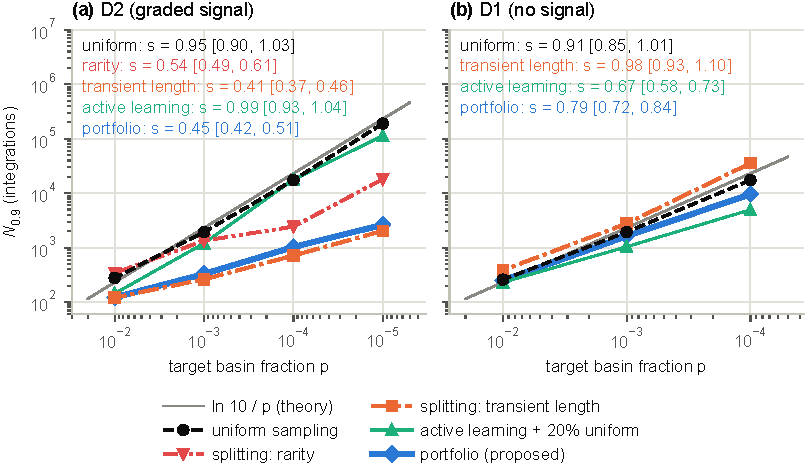
\includegraphics[width=\textwidth]{fig23_scaling_p.pdf}
\caption{Detection cost $N_{0.9}$ versus basin measure $p$ ($n=6$, $R=100$), with scaling exponents $s$ ($N_{0.9}\propto p^{-s}$) and 95\% intervals. (a) Family D2 with a signal on all scales. (b) Family D1 without a signal. ``Rarity'' is splitting by the multidimensional rarity of the fingerprint (Section~\ref{app:ablation}). Thin gray line: $\ln10/p$.}
\label{fig:scalp}
\end{figure}

\subsection{Rare targets of levels A and B}\label{sec:rare_ab}

On the three rare targets with a transient signal, Chua~II, SE11, and LE1, the portfolio outperforms uniform sampling by factors of 7.4, 3.1, and 6.2, with the lower ends of the 95\% intervals above 1 (\cref{tab:gains}, \cref{fig:pn}); with nullcline sampling (channel C), it also gains on Chua~I (4.4). On SE11 and LE1, these gains stay within the escape-time bounds of \cref{cor:channels} (54 and 230), which are moderate because $\mu(Q_\infty)$ of a single unit is not small; the large gains of \cref{sec:coupled} arise where the bound itself is large. On Chua~II, all trajectories are bounded, and escape times are worth at most 2.56; the gain of 7.4 comes from the settling part $D$ of $\xi$, since splitting along the escape step alone gains 1.04, and splitting along $\xi$ gains 5.05 (Section~\ref{sec:ablation_main}). On LE1, splitting is the best single arm (8.3), whereas active learning loses to uniform sampling (0.48): the long boundary between convergence to the continuum of equilibria and escape attracts the queries, and the target adjoins this boundary only along a small part of it. On the Jafari cycle, the Jafari chaos, and the Huynh map, the portfolio loses or gains little, as the cost model predicts (\cref{sec:failures}), and stays within the bound of \cref{prop:portfolio}: 0.43, 0.42, and 1.40. Zelinka's DE, which is given the size of the target, is nowhere significantly better than uniform sampling and loses by factors of 4.3 and 3.4 on the Jafari chaos and cycle, respectively. On the five Jiang maps that were searched ($p\approx0.03$--$0.07$), all strategies are close to uniform sampling, because the target is often found within the initial sample. Ablations, hyperparameter variants, and tests of the integration horizon are reported in Section~\ref{app:ablation}: no variant brings the gain below 1, and scaling both integration windows by 0.5 or 2 keeps the gains within a factor of 1.7.

\begin{table}[tbhp]
\caption{Gains $G_{0.9}=N^0_{0.9}/N_{0.9}$ ($R=100$), with 95\% bootstrap intervals for splitting and the portfolio (all intervals and the Jiang maps: Table~\ref{tab:gainsfull}); $p$ is the combined measure of the two symmetric attractors where there are two. AL: active learning with a 20\% uniform share; +NC: portfolio with nullcline sampling; ``---'': not run.}
\label{tab:gains}
\centering\scriptsize
\setlength{\tabcolsep}{3pt}
\begin{tabular}{lrrrrrrr}
\toprule
System & $p$ & $N^0_{0.9}$ & DE & Splitting & AL & Portfolio & +NC \\
\midrule
Chua I & 0.035 & 66 & 0.60 & 1.20 \ci{0.92}{1.77} & 1.23 & 1.24 \ci{0.94}{1.77} & 4.42 \\
Chua II & 0.0027 & 818 & 0.84 & 5.05 \ci{4.13}{7.07} & 3.16 & 7.36 \ci{6.09}{10.2} & 7.64 \\
SE11 & 0.0079 & 317 & 0.95 & 2.53 \ci{1.95}{2.86} & 3.62 & 3.10 \ci{2.46}{3.70} & 3.56 \\
LE1 & 0.0016 & 1617 & 1.31 & 8.29 \ci{6.35}{12.3} & 0.48 & 6.24 \ci{3.76}{10.0} & 4.62 \\
Jafari, cycle & 0.009 & 219 & 0.29 & 0.29 \ci{0.19}{0.53} & 0.88 & 0.43 \ci{0.29}{0.78} & 0.32 \\
Huynh 2019 & 0.0091 & 221 & 0.45 & 1.36 \ci{0.79}{2.42} & 0.82 & 1.40 \ci{1.16}{2.54} & --- \\
Jafari, chaos & $(2$--$5)\times10^{-4}$ & 5265 & 0.23 & 0.22 \ci{0.15}{0.28} & 1.08 & 0.42 \ci{0.29}{0.58} & 0.27 \\
\bottomrule
\end{tabular}
\end{table}

\begin{figure}[tbhp]
\centering
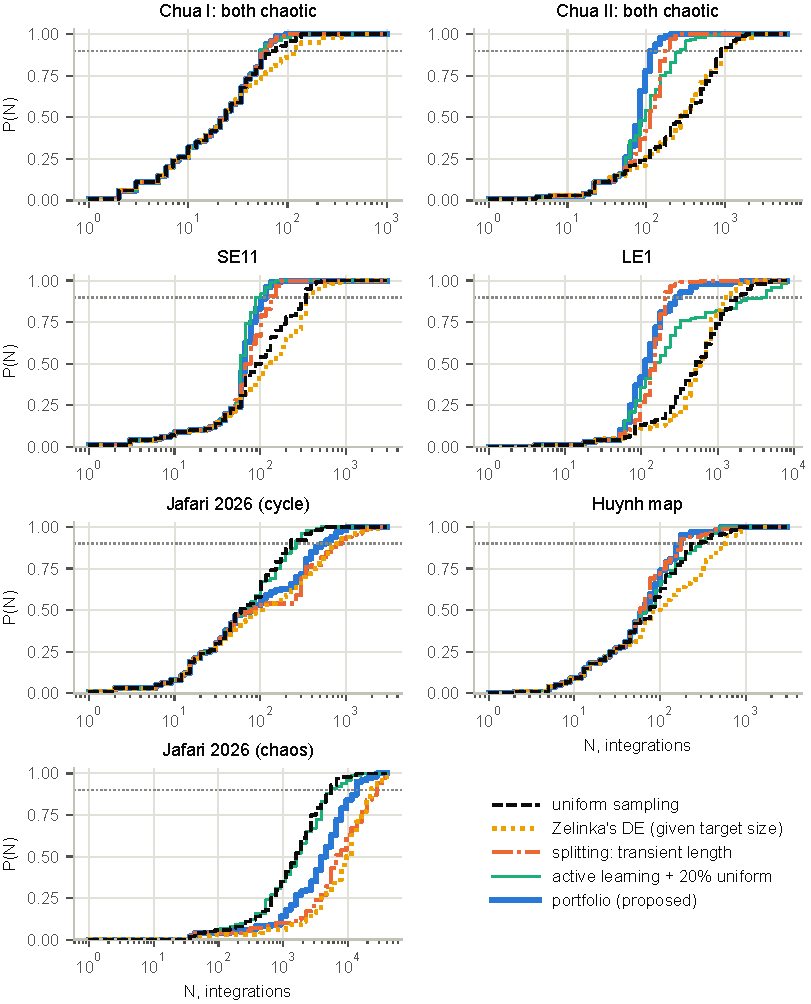
\includegraphics[width=\textwidth]{fig21_pn_levelAB.pdf}
\caption{Detection probability $P(N)$ versus the number of integrations for rare targets of levels A and B ($R=100$); the dotted line is the 0.9 level, and for $N\le50$ all curves coincide by construction. On Chua~II, SE11, and LE1, the portfolio (thick line) lies to the left of uniform sampling over the whole range; on the Jafari cycle and chaos, it lies to the right, within the guaranteed factor $1/\theta$.}
\label{fig:pn}
\end{figure}

\subsection{Stagger-and-step as an arm of the portfolio}\label{sec:sas}

A single stagger-and-step chain on the coordinate $\xi$ is stronger than both the splitting arm and the portfolio where the signal is present (10.1 on Chua~II, $s=0.32$ on D2). Having no uniform share, it falls below the bound of the portfolio where the coordinate is deceptive or absent (0.16 on the Jafari cycle; 60\% success on D1). \Cref{cor:sas} turns it into a safe arm. Since the portfolio evaluates points in rounds, we added an arm of $n_c=10$ chains, each contributing one point per round, with shares $\omega_{\rm sas}=0.2$ for the chains, 0.2 for splitting, 0.4 for active learning, and $\theta=0.2$ ($c=50$). We also replaced the splitting arm with the chains; \cref{tab:psas} gives the results ($R=50$). The bound of \cref{cor:sas} held on all twelve problems. Where the chains fail (the Jafari cycle and chaos, D1), the portfolio with them stays within the guarantee, and the variant without splitting is the most robust there (0.94, 0.70, and 1.31). On D2, the ten-chain arm alone has $s=0.31$, the portfolio with it $0.43$, and the portfolio with chains instead of splitting $0.51$. The exponent statement of \cref{cor:sas} is asymptotic: over $p=10^{-2}$--$10^{-5}$, the cost of the portfolio with the chains rises from 0.6 to 1.4 times that of the chains alone, still far below the ceiling $1/\omega_{\rm sas}=5$, so the measured exponent exceeds that of the chains. Across the portfolio variants of \cref{tab:psas}, the choice of the arm changes the gains on D2 by factors of up to about 3, not their order of growth. Ten chains in parallel are weaker than one chain on Chua~II and on D2 at the same total budget, because each chain advances ten times more slowly. In sequential evaluation, a single chain alternating with a uniform share $\theta$ would, by \cref{prop:portfolio}, cost at most $(N_{0.9}(\text{chain})+c)/(1-\theta)$, about 1.25 times the chain where it works, and at most $(N^0_{0.9}+c)/\theta$ where it fails.

\begin{table}[tbhp]
\caption{Stagger-and-step and the portfolio: gains $G_{0.9}$ against the fixed uniform reference $N^0_{0.9}$ (new variants: $R=50$; bootstrap intervals in the data archive). Portfolio: three arms, from \cref{tab:gains,tab:scaling} and, for D1, Table~\ref{tab:stagger} ($R=100$). One chain: single stagger-and-step chain, from Table~\ref{tab:stagger}. Chains: the ten-chain arm alone. +SAS: portfolio with the ten-chain arm added; SAS for split.: chains instead of splitting. A percentage gives the fraction of successful runs where this fraction is below 90\%. Last row: exponent $s$ on D2 over $p=10^{-2}$--$10^{-5}$.}
\label{tab:psas}
\centering\scriptsize
\setlength{\tabcolsep}{4pt}
\begin{tabular}{lrrrrrr}
\toprule
Problem & $N^0_{0.9}$ & Portfolio & One chain & Chains & +SAS & SAS for split. \\
\midrule
Chua I & 66 & 1.24 & 1.67 & 0.78 & 1.24 & 1.28 \\
Chua II & 818 & 7.36 & 10.1 & 2.69 & 4.92 & 3.24 \\
SE11 & 317 & 3.10 & 2.90 & 1.84 & 2.44 & 3.22 \\
LE1 & 1617 & 6.24 & 5.85 & 4.28 & 6.58 & 2.18 \\
Jafari, cycle & 219 & 0.43 & 0.16 & 0.27 & 0.47 & 0.94 \\
Huynh 2019 & 221 & 1.40 & 0.93 & 1.02 & 1.16 & 0.86 \\
Jafari, chaos & 5265 & 0.42 & 0.26 & 0.23 & 0.38 & 0.70 \\
D1, $p=10^{-3}$ & 1932 & 1.19 & 60\% & 74\% & 0.90 & 1.31 \\
D2, $p=10^{-2}$ & 277 & 2.27 & 2.14 & 0.99 & 1.65 & 1.51 \\
D2, $p=10^{-3}$ & 1932 & 5.87 & 6.99 & 3.46 & 3.65 & 1.79 \\
D2, $p=10^{-4}$ & 17\,416 & 17.0 & 34.5 & 15.4 & 13.2 & 5.29 \\
D2, $p=10^{-5}$ & 189\,765 & 72.0 & 155 & 81.3 & 57.0 & 29.7 \\
\midrule
$s$ on D2 & & 0.45 & 0.32 & 0.31 & 0.43 & 0.51 \\
\bottomrule
\end{tabular}
\end{table}

\subsection{Cost in integrator steps and wall time}\label{sec:cost}

A count of integrations is a fair measure of cost only if all integrations cost about the same, a condition that fails when trajectories escape: an escaping trajectory stops at the step of escape, and the method concentrates on long-lived trajectories. We therefore measured the cost of the two-stage configuration of the portfolio in integrator steps and wall time against uniform sampling with the same evaluation (\cref{tab:cost}, \cref{fig:cost}); for coupled systems, the products of the attractors of single units other than the target are declared known (product templates). The problems fall into two groups. In systems where most trajectories escape quickly (Chua~I, SE11, LE1, D2, coupled SE11), the portfolio spends 2--300 times more steps per evaluation than uniform sampling, because it selects the long transients that lead toward the target, whereas most uniform points escape within a few steps. The gain in integrations then shrinks by a factor of 3--300 when measured in steps, and the portfolio gains in time with statistical significance only where the gain in integrations is very large, on three coupled copies of SE11 ($G_N=3600$, $G_T=29$). In systems with bounded trajectories (Chua~II and its copies), the steps per evaluation of the portfolio and of uniform sampling are close, and the gain carries over to time: 4.1 on Chua~II, 68 on the coupled circuits, and 130--150 on the uncoupled copies. Product templates matter: on three coupled copies of SE11, they lower $N_{0.9}$ from 3500 to 2100 and raise $G_T$ from 9 to 29. They presuppose, however, that the attractors of the units are known; otherwise, the gain without them applies, 2200 in integrations and 9 in time. This gain differs from the 1435 of \cref{tab:coupled} because two-stage evaluation computes $\xi$ of stopped trajectories over a shorter window and because these runs are few. These time gains were measured with four threads per process; on one thread (Table~\ref{tab:time}), they are 27 on the coupled circuits and 5.7 on Chua~II. Against uniform sampling with recurrence-based stopping as in Attractors.jl~\cite{DatserisWagemakers2022,Datseris2023Framework}, which evaluates bounded trajectories about three times faster, these one-thread gains fall to 10 and 1.8, both still significant (Section~\ref{sec:recurrence}).

\begin{table}[tbhp]
\caption{Cost of the two-stage configuration of the portfolio relative to uniform sampling with the same evaluation at a fixed reference cost ($R=20$; three copies of Chua~II: $R=10$, 9 successful runs): mean integrator steps per evaluation and gains in integrations ($G_N$), steps ($G_S$), and wall time ($G_T$, four threads per process), with 95\% bootstrap intervals for $G_S$ and $G_T$.}
\label{tab:cost}
\centering\scriptsize
\setlength{\tabcolsep}{3pt}
\begin{tabular}{lrrrrrr}
\toprule
Problem & $p$ & \multicolumn{2}{c}{Steps per evaluation} & $G_N$ & $G_S$ & $G_T$ \\
 & & Uniform & Portfolio & & & \\
\midrule
Chua I & 0.033 & $2.6\times10^{4}$ & $4.6\times10^{4}$ & 1.2 & 0.36 \ci{0.27}{1.4} & 0.31 \ci{0.24}{1.1} \\
SE11 & 0.0077 & 1139 & 3681 & 4.5 & 1.0 \ci{0.84}{1.3} & 0.85 \ci{0.78}{1.1} \\
LE1 & 0.0013 & 334 & $1.1\times10^{4}$ & 3.9 & 0.095 \ci{0.018}{0.65} & 0.14 \ci{0.029}{0.76} \\
D2, $p=10^{-4}$ & $1.0\times10^{-4}$ & 14 & 1169 & 17 & 0.18 \ci{0.12}{0.26} & 0.26 \ci{0.18}{0.54} \\
D2, $p=10^{-5}$ & $1.0\times10^{-5}$ & 2 & 616 & 100 & 0.35 \ci{0.052}{2.1} & 1.5 \ci{0.27}{3.1} \\
2 coupled SE11 & $5.5\times10^{-5}$ & 117 & 3694 & 61 & 1.2 \ci{1.1}{3.8} & 1.1 \ci{0.70}{3.0} \\
3 coupled SE11 & $3.5\times10^{-7}$ & 45 & 3418 & 3600 & 41 \ci{31}{57} & 29 \ci{22}{44} \\
Chua II & 0.0026 & $8.7\times10^{4}$ & $9.7\times10^{4}$ & 7.3 & 6.1 \ci{4.8}{8.6} & 4.1 \ci{2.9}{6.3} \\
2 Chua II, $\epsilon=0.1$ & $2.3\times10^{-5}$ & $3.0\times10^{5}$ & $3.4\times10^{5}$ & 55 & 49 \ci{20}{87} & 68 \ci{14}{110} \\
2 Chua II, $\epsilon=0$ & $7.3\times10^{-6}$ & $1.7\times10^{5}$ & $1.9\times10^{5}$ & 190 & 160 \ci{110}{230} & 130 \ci{91}{200} \\
3 Chua II, $\epsilon=0$ & $2.0\times10^{-8}$ & $1.7\times10^{5}$ & $2.3\times10^{5}$ & 360 & 270 \ci{0}{740} & 150 \ci{0}{340} \\
\bottomrule
\end{tabular}
\end{table}

\begin{figure}[tbhp]
\centering
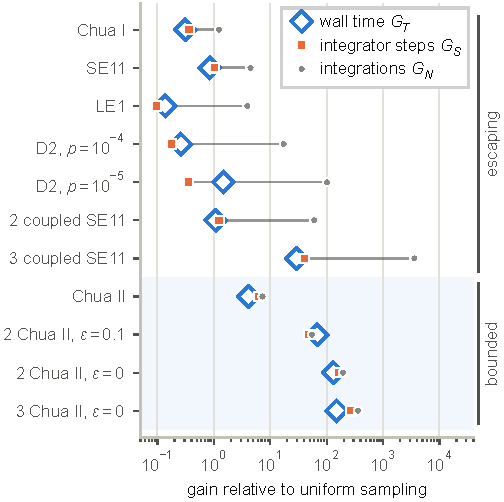
\includegraphics[width=0.62\textwidth]{fig30_cost_gains.pdf}
\caption{Gain of the portfolio relative to uniform sampling, both with two-stage evaluation, in integrations ($G_N$), integrator steps ($G_S$), and wall time ($G_T$) for escaping systems (top group) and bounded systems (bottom group). Dashed line: $G=1$.}
\label{fig:cost}
\end{figure}

\subsection{A hidden attractor born of the coupling}\label{sec:newattr}

The enumeration of the regimes of two coupled Chua~II circuits ($\epsilon=0.1$) revealed a regime that a single circuit does not have (\cref{fig:newattr}): one circuit stays on the large cycle, and the other hops chaotically between the regions of the two hidden attractors HA$_a$ and HA$_b$, which never merge in the single circuit at these parameters~\cite{Stankevich2017}. Dynamically, it is the chaotic response of the second circuit to the nearly periodic drive of the first, with weak feedback; chaos in a periodically driven Chua circuit is classical~\cite{Murali1991DrivenChua}, but here the drive is generated by another copy of the same circuit, and the coupled system is autonomous. The regime passes the verification protocol: sixteen perturbed copies stay on it for $10^5$ time units (four of them for $10^6$) with RK4, eight copies integrated with DOP853 for $2\times10^4$ time units end on the same template, the template is unchanged at $\Delta t/2$, and the largest Lyapunov exponent over windows of 100 time units is $0.095\pm0.052$. It is hidden: none of the $2\times10^5$ trajectories per radius started in the $10^{-3}L$ and $10^{-2}L$ neighborhoods of the nine equilibria and along their unstable directions reaches it ($h_\varepsilon<1.5\times10^{-5}$). Continuation in the coupling strength shows its birth: for $\epsilon<0.045$, the second circuit oscillates periodically near one of its stable equilibria; at $\epsilon\approx0.045$, these branches merge into the chaotic hopping; $\lambda$ grows almost linearly to 0.35 at $\epsilon=0.46$, with periodic windows at $\epsilon=0.09$ and 0.47; and at $\epsilon\approx0.5$, the branches merge with the synchronized cycle. Coupled Chua circuits with hidden attractors have been studied in the context of synchronization~\cite{Stankevich2017,Kuznetsov2023Chua}, but this regime does not appear to have been reported. It is hidden but not rare (0.4\%--1\% of the region per symmetric branch at all $\epsilon$), so the value of the method here lies in enumeration with verification rather than in speed (\cref{tab:newattr}).

\begin{figure}[tbhp]
\centering
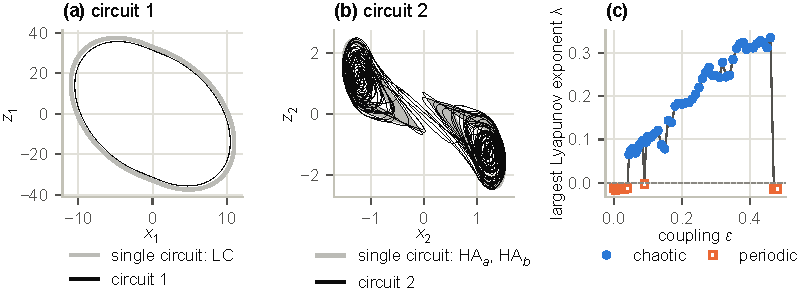
\includegraphics[width=\textwidth]{fig31_new_attractor.pdf}
\caption{Hidden attractor of two coupled Chua~II circuits born of the coupling ($\epsilon=0.1$). (a) Circuit 1 in the projection $(x_1,z_1)$, together with the cycle of the single circuit. (b) Circuit 2 in $(x_2,z_2)$, together with the hidden attractors HA$_a$ and HA$_b$ of the single circuit (gray). (c) Largest Lyapunov exponent versus the coupling strength, from continuation in $\epsilon$.}
\label{fig:newattr}
\end{figure}

\begin{table}[tbhp]
\caption{Finding the coupling-born attractor (basin fraction 0.016 for the two branches combined): integrations to detection (0.9 quantile and median over $R=20$ runs; for uniform sampling, $\ln10/p=144$) and wall time $T_{0.9}$ on one thread with full integration, two-stage evaluation, and recurrence-based stopping (Attractors.jl). ``From equilibria'': the standard procedure. Product state: the initial condition built from the cycle and HA$_a$ of the single circuit.}
\label{tab:newattr}
\centering\scriptsize
\begin{tabular}{lrrrrr}
\toprule
Method & $N_{0.9}$ & Median & \multicolumn{3}{c}{$T_{0.9}$, s} \\
 & & & full & two-stage & recurrence \\
\midrule
From equilibria & never & --- & --- & --- & --- \\
Uniform & 230 & 18 & 28 & 17 & 6.4 \\
Portfolio & 81 & 18 & --- & 8.1 & --- \\
Product state & 1 & 1 & 0.07 & --- & --- \\
\bottomrule
\end{tabular}
\end{table}

\subsection{Failures and limits}\label{sec:failures}

The failures delineate the domain of applicability and are the cases predicted by \cref{prop:cost}.
\textbf{Deceptive coordinate.} In the Jafari chaos, almost all trajectories escape by slow drift, and the longest escape times occur in the region of slow drift rather than near the attractor; splitting is 4.5 times slower than uniform sampling ($e_l<1$), and the portfolio stays within the bound (0.42). In an enlarged region, slowly returning trajectories make the coordinate deceptive even for Chua~II (Section~\ref{app:enlarged}).
\textbf{Escape without a gradient of duration.} For the Jafari cycle, the escape time is set by slow drift, and for the Huynh map, the escape times are discrete; the target is an island among escaping trajectories, and the transients do not point toward it.
\textbf{A long boundary of known basins that the target touches only along a small part} (LE1): active learning has a median cost 3.7 times lower than that of uniform sampling but a heavy tail (16 of 100 runs above $N^0_{0.9}$, two of them without a hit); in the portfolio, the tail is bounded.
\textbf{Time resolution.} The discretization limit at very small $p$ and the cheap nontarget trajectories of escaping systems are two faces of the same constraint: the coordinate and the cost are both set by integrator steps.
\textbf{Single adaptive strategies} produce heavy tails or fail in a fraction of runs (Section~\ref{app:ablation}); the uniform share of the portfolio removes exactly these tails.
